\subsection{Enumeration types}
\label{subsec:library_of_transformations:type_level_transformations:enumeration_types}

\begin{figure}[H]
    \centering
    \begin{subfigure}{0.25\textwidth}
        \centering
        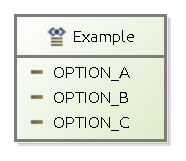
\includegraphics{images/05_library_of_transformations/02_type_level_transformations/04_enumeration_types/enum_type.pdf}
        \caption{$Tm_{Enum}$ with \\$name = .\type{Example}$ and \\$values = \{ \type{OPTION\_A},$\\$ \type{OPTION\_B}, \type{OPTION\_C} \}$}
        \label{fig:library_of_transformations:type_level_transformations:enumeration_types:visualisation:ecore}
    \end{subfigure}
    \\
    \begin{subfigure}{0.65\textwidth}
        \centering
        % To use this figure in your LaTeX document
% import the package groove/resources/groove2tikz.sty
%
\begin{tikzpicture}[scale=\tikzscale,name prefix=test-]
\node[abstract_node] (n1) at (3.160, -0.665) {\ml{\textit{\textbf{Example}}}};
\node[type_node] (n0) at (1.550, -1.875) {\ml{\textbf{Example\$OPTION\_A}}};
\node[type_node] (n2) at (3.160, -1.875) {\ml{\textbf{Example\$OPTION\_B}}};
\node[type_node] (n3) at (4.760, -1.875) {\ml{\textbf{Example\$OPTION\_C}}};

\path[subtype_edge] (n0)  --  (n1) ;
\path[subtype_edge](n2.north -| 3.160, -0.665) --  (n1) ;
\path[subtype_edge] (n3)  --  (n1) ;
\end{tikzpicture}

        \caption{$TG_{EnumNodes}$ with $name = .\type{Example}$ and\\$values = \{ \type{OPTION\_A}, \type{OPTION\_B}, \type{OPTION\_C} \}$}
        \label{fig:library_of_transformations:type_level_transformations:enumeration_types:visualisation:groove_nodes}
    \end{subfigure}
    \begin{subfigure}{0.25\textwidth}
        \centering
        % To use this figure in your LaTeX document
% import the package groove/resources/groove2tikz.sty
%
\begin{tikzpicture}[scale=\tikzscale,name prefix=test-]
\node[type_node] (n1) at (3.160, -0.665) {\ml{\textbf{Example}\\\textit{OPTION\_A}\\\textit{OPTION\_B}\\\textit{OPTION\_C}}};

\end{tikzpicture}

        \caption{$TG_{EnumFlags}$ with \\$name = .\type{Example}$ and \\$values = \{ \type{OPTION\_A},$\\$ \type{OPTION\_B}, \type{OPTION\_C} \}$}
        \label{fig:library_of_transformations:type_level_transformations:enumeration_types:visualisation:groove_flags}
    \end{subfigure}
    \caption{Visualisations of the transformations of enumeration types}
    \label{fig:library_of_transformations:type_level_transformations:enumeration_types:visualisation}
\end{figure}

This section will define the transformation of an enumeration type. Within this transformation, a new enumeration type is introduced, including its possible values. The Ecore type model that introduces such a subclass is defined as follows:

\begin{defin}[Type model $Tm_{Enum}$]
\label{defin:library_of_transformations:type_level_transformations:enumeration_types:tmod_enum}
Let $Tm_{Enum}$ be the type model containing a enumeration type with identifier $name$. The values of this enumeration type are defined as part of sequence $values$. $Tm_{Enum}$ is defined as:
\begin{align*}
Class =\ &\{\} \\
Enum =\ &\{name\} \\
UserDataType =\ &\{\} \\
Field =\ &\{\} \\
\mathrm{FieldSig} =\ &\{\} \\
EnumValue =\ &\{ (name, v) \mid v \in values \} \\
Inh =\ &\{\} \\
Prop =\ &\{\} \\
Constant =\ &\{\} \\
\mathrm{ConstType} =\ &\{\}
\end{align*}
\isabellelref{tmod_enum}{Ecore-GROOVE-Mapping-Library.EnumType}
\end{defin}

\begin{thm}[Correctness of $Tm_{Enum}$]
\label{defin:library_of_transformations:type_level_transformations:enumeration_types:tmod_enum_correct}
$Tm_{Subclass}$ (\cref{defin:library_of_transformations:type_level_transformations:enumeration_types:tmod_enum}) is a consistent type model in the sense of \cref{defin:formalisations:ecore_formalisation:type_models:type_model_consistency}.
\isabellelref{tmod_enum_correct}{Ecore-GROOVE-Mapping-Library.EnumType}
\end{thm}

A visual representation of $Tm_{Enum}$ with $.\type{Example}$ as identifier for the new enumeration type and $\type{OPTION\_A}$, $\type{OPTION\_B}$ and $\type{OPTION\_C}$ as its values can be seen in \cref{fig:library_of_transformations:type_level_transformations:enumeration_types:visualisation:ecore}. The correctness proof of $Tm_{Enum}$ is trivial, and therefore not included here. The proof can be found as part of the Isabelle validated proofs.

In order to make composing transformation functions possible, $Tm_{Enum}$ should be compatible with the type model it is combined with.

\begin{thm}[Correctness of $\mathrm{combine}(Tm, Tm_{Enum})$]
\label{defin:library_of_transformations:type_level_transformations:enumeration_types:tmod_enum_combine_correct}
Assume a type model $Tm$ that is consistent in the sense of \cref{defin:formalisations:ecore_formalisation:type_models:type_model_consistency}. Then $Tm$ is compatible with $Tm_{Enum}$ (in the sense of \cref{defin:transformation_framework:type_models_and_type_graphs:combining_type_models:compatibility}) if:
\begin{itemize}
    \item The identifier of the enumeration type in $Tm_{Enum}$ is not yet an identifier for a class, enumeration type or user-defined data type in $Tm$;
    \item The identifier of the enumeration type in $Tm_{Enum}$ is not in the namespace of any class, enumeration type or user-defined data type in $Tm$;
    \item None of the identifiers in any class, enumeration type or user-defined data type in $Tm$ is in the namespace of the enumeration type in $Tm_{Enum}$.
\end{itemize}
\isabellelref{tmod_enum_combine_correct}{Ecore-GROOVE-Mapping-Library.EnumType}
\end{thm}

\begin{proof}
Use \cref{defin:transformation_framework:type_models_and_type_graphs:combining_type_models:tmod_combine_merge_correct}. It is possible to show that all assumptions hold. Now we have shown that $\mathrm{combine}(Tm, Tm_{Enum})$ is consistent in the sense of \cref{defin:formalisations:ecore_formalisation:type_models:type_model_consistency}.
\end{proof}

The definitions and theorems for a regular subclass within Ecore are now complete. 

\subsubsection{Encoding as node type}

A possible encoding for enumeration types in Ecore is using node types in GROOVE. In this case, the enumeration type itself is transformed into an abstract node type. Each value of the enumeration type is converted to its own node type, extending the abstract node type. The encoding corresponding to $Tm_{Enum}$ can then be represented as $TG_{EnumNodes}$, defined in the following definition:

\begin{defin}[Type graph $TG_{EnumNodes}$]
\label{defin:library_of_transformations:type_level_transformations:enumeration_types:tg_enum_as_node_types}
Let $TG_{EnumNodes}$ be a type graph containing multiple node types. The first node type encodes the enumeration type $name$. The other node types encode the $values$ of enumeration type $name$. $TG_{EnumNodes}$ is defined as:
\begin{align*}
NT =\ &\{\mathrm{ns\_\!to\_\!list}(name)\} \cup \{ \mathrm{ns\_\!to\_\!list}(name) \append \langle v \rangle \mid v \in values \} \\
ET =\ &\{\} \\
\!\!\sqsubseteq\ =\ &\{(\mathrm{ns\_\!to\_\!list}(name), \mathrm{ns\_\!to\_\!list}(name))\}\ \cup \\&
\{(\mathrm{ns\_\!to\_\!list}(name) \append \langle v \rangle, \mathrm{ns\_\!to\_\!list}(name) \append \langle v \rangle) \mid v \in values \}\ \cup \\&
\{(\mathrm{ns\_\!to\_\!list}(name) \append \langle v \rangle, \mathrm{ns\_\!to\_\!list}(name)) \mid v \in values \} \\
abs =\ &\{\mathrm{ns\_\!to\_\!list}(name)\} \\
\mathrm{mult} =\ &\{\} \\
contains =\ &\{\}
\end{align*}
\isabellelref{tg_enum_as_node_types}{Ecore-GROOVE-Mapping-Library.EnumType}
\end{defin}

\begin{thm}[Correctness of $TG_{EnumNodes}$]
\label{defin:library_of_transformations:type_level_transformations:enumeration_types:tg_enum_as_node_types_correct}
$TG_{EnumNodes}$ (\cref{defin:library_of_transformations:type_level_transformations:enumeration_types:tg_enum_as_node_types}) is a valid type graph in the sense of \cref{defin:formalisations:groove_formalisation:type_graphs:type_graph_validity}.
\isabellelref{tg_enum_as_node_types_correct}{Ecore-GROOVE-Mapping-Library.EnumType}
\end{thm}

A visual representation of $TG_{EnumNodes}$ with $.\type{Example}$ as identifier for the encoded enumeration type and $\type{OPTION\_A}$, $\type{OPTION\_B}$ and $\type{OPTION\_C}$ as its values can be seen in \cref{fig:library_of_transformations:type_level_transformations:enumeration_types:visualisation:groove_nodes}. Please note that in this visualisation, the sequences are concatenated using the dollar sign $\$$. The correctness proof of $TG_{EnumNodes}$ is trivial, and therefore not included here. The proof can be found as part of the Isabelle validated proofs.

In order to make composing transformation functions possible, $TG_{EnumNodes}$ should be compatible with the type graph it is combined with.

\begin{thm}[Correctness of $\mathrm{combine}(TG, TG_{EnumNodes})$]
\label{defin:library_of_transformations:type_level_transformations:enumeration_types:tg_enum_as_node_types_combine_correct}
Assume a type graph $TG$ that is valid in the sense of \cref{defin:formalisations:groove_formalisation:type_graphs:type_graph_validity}. Then $TG$ is compatible with $TG_{EnumNodes}$ (in the sense of \cref{defin:transformation_framework:type_models_and_type_graphs:combining_type_graphs:compatibility}) if:
\begin{itemize}
    \item There are no shared node types between $TG_{EnumNodes}$ and $TG$.
\end{itemize}
\isabellelref{tg_enum_as_node_types_combine_correct}{Ecore-GROOVE-Mapping-Library.EnumType}
\end{thm}

\begin{proof}
Use \cref{defin:transformation_framework:type_models_and_type_graphs:combining_type_graphs:tg_combine_merge_correct}. It is possible to show that all assumptions hold. Now we have shown that $\mathrm{combine}(TG, TG_{EnumNodes})$ is valid in the sense of \cref{defin:formalisations:groove_formalisation:type_graphs:type_graph_validity}.
\end{proof}

The next definitions define the transformation function from $Tm_{Enum}$ to $TG_{EnumNodes}$:

\begin{defin}[Transformation function $f_{EnumNodes}$]
\label{defin:library_of_transformations:type_level_transformations:enumeration_types:tmod_enum_to_tg_enum_as_node_types}
The transformation function $f_{EnumNodes}(Tm)$ is defined as:
\begin{align*}
NT =\ &\{\mathrm{ns\_\!to\_\!list}(e) \mid e \in Enum_{Tm}\} \cup \{\mathrm{ns\_\!to\_\!list}(e) \append \langle v \rangle \mid (e, v) \in EnumValue_{Tm}\} \\
ET =\ &\{\} \\
\!\!\sqsubseteq\ =\ &\{(\mathrm{ns\_\!to\_\!list}(e_1), \mathrm{ns\_\!to\_\!list}(e_2)) \mid e_1 \in Enum_{Tm} \land e_2 \in Enum_{Tm} \}\ \cup \\&
\{(\mathrm{ns\_\!to\_\!list}(i) \append \langle j \rangle, \mathrm{ns\_\!to\_\!list}(i) \append \langle j \rangle) \mid (i, j) \in EnumValue_{Tm} \}\ \cup \\&
\{(\mathrm{ns\_\!to\_\!list}(i) \append \langle j \rangle, \mathrm{ns\_\!to\_\!list}(e)) \mid (i, j) \in EnumValue_{Tm} \land e \in Enum_{Tm} \} \\
abs =\ &\{\} \\
\mathrm{mult} =\ &\{\} \\
contains =\ &\{\}
\end{align*}
\isabellelref{tmod_enum_to_tg_enum_as_node_types}{Ecore-GROOVE-Mapping-Library.EnumType}
\end{defin}

\begin{thm}[Correctness of $f_{EnumNodes}$]
\label{defin:library_of_transformations:type_level_transformations:enumeration_types:tmod_enum_to_tg_enum_as_node_types_func}
$f_{EnumNodes}(Tm)$ (\cref{defin:library_of_transformations:type_level_transformations:enumeration_types:tmod_enum_to_tg_enum_as_node_types}) is a valid transformation function in the sense of \cref{defin:transformation_framework:type_models_and_type_graphs:combining_transformation_functions:transformation_function_type_model_type_graph} transforming $Tm_{Enum}$ into $TG_{EnumNodes}$.
\isabellelref{tmod_enum_to_tg_enum_as_node_types_func}{Ecore-GROOVE-Mapping-Library.EnumType}
\end{thm}

The proof of the correctness of $f_{EnumNodes}$ will not be included here. Instead, it can be found in the validated Isabelle theories.

Finally, to complete the transformation, the transformation function that transforms $TG_{EnumNodes}$ into $Tm_{Enum}$ is defined:

\begin{defin}[Transformation function $f'_{EnumNodes}$]
\label{defin:library_of_transformations:type_level_transformations:enumeration_types:tg_enum_as_node_types_to_tmod_enum}
The transformation function $f'_{EnumNodes}(TG, name)$ is defined as:
\begin{align*}
Class =\ &\{\} \\
Enum =\ &\{\mathrm{list\_\!to\_\!ns}(n) \mid n \in NT_{TG} \land n = \mathrm{id\_\!to\_\!name}(name)\} \\
UserDataType =\ &\{\} \\
Field =\ &\{\} \\
\mathrm{FieldSig} =\ &\{\} \\
EnumValue =\ &\{(\mathrm{list\_\!to\_\!ns}(e), v) \mid e \append \langle v \rangle \in NT_{TG} \land e \append \langle v \rangle \neq \mathrm{id\_\!to\_\!name}(name) \} \\
Inh =\ &\{\} \\
Prop =\ &\{\} \\
Constant =\ &\{\} \\
\mathrm{ConstType} =\ &\{\}
\end{align*}
\isabellelref{tg_enum_as_node_types_to_tmod_enum}{Ecore-GROOVE-Mapping-Library.EnumType}
\end{defin}

\begin{thm}[Correctness of $f'_{EnumNodes}$]
\label{defin:library_of_transformations:type_level_transformations:enumeration_types:tg_enum_as_node_types_to_tmod_enum_func}
$f'_{EnumNodes}(TG, name)$ (\cref{defin:library_of_transformations:type_level_transformations:enumeration_types:tg_enum_as_node_types_to_tmod_enum}) is a valid transformation function in the sense of \cref{defin:transformation_framework:type_models_and_type_graphs:combining_transformation_functions:transformation_function_type_graph_type_model} transforming $TG_{EnumNodes}$ into $Tm_{Enum}$.
\isabellelref{tg_enum_as_node_types_to_tmod_enum_func}{Ecore-GROOVE-Mapping-Library.EnumType}
\end{thm}

Once more, the correctness proof is not included here but can be found in the validated Isabelle proofs of this thesis.

\subsubsection{Encoding as flags}

Another possible encoding for enumeration types in Ecore is using flags in GROOVE. In this case, the enumeration type itself is transformed into a regular node type. Each value of the enumeration type is converted to a flag on this node type. The encoding corresponding to $Tm_{Enum}$ can then be represented as $TG_{EnumFlags}$, defined in the following definition:

\begin{defin}[Type graph $TG_{EnumFlags}$]
\label{defin:library_of_transformations:type_level_transformations:enumeration_types:tg_enum_as_flags}
Let $TG_{EnumFlags}$ be a type graph containing a single node type which encodes the enumeration type $name$. The flags on the node type of $name$ encode the different $values$. $TG_{EnumFlags}$ is defined as:
\begin{align*}
NT =\ &\{\mathrm{ns\_\!to\_\!list}(name)\} \\
ET =\ &\{ (\mathrm{ns\_\!to\_\!list}(name), \langle v \rangle, \mathrm{ns\_\!to\_\!list}(name)) \mid v \in values \}\\
\!\!\sqsubseteq\ =\ &\{(\mathrm{ns\_\!to\_\!list}(name), \mathrm{ns\_\!to\_\!list}(name))\} \\
abs =\ &\{\} \\
\mathrm{mult}(e) =\ &\begin{cases}
    (0..1, 0..1) &\mathrm{if}\ e \in ET_{TG_{EnumFlags}}
\end{cases}\\
contains =\ &\{\}
\end{align*}
\isabellelref{tg_enum_as_flags}{Ecore-GROOVE-Mapping-Library.EnumType}
\end{defin}

\begin{thm}[Correctness of $TG_{EnumFlags}$]
\label{defin:library_of_transformations:type_level_transformations:enumeration_types:tg_enum_as_flags_correct}
$TG_{EnumFlags}$ (\cref{defin:library_of_transformations:type_level_transformations:enumeration_types:tg_enum_as_flags}) is a valid type graph in the sense of \cref{defin:formalisations:groove_formalisation:type_graphs:type_graph_validity}.
\isabellelref{tg_enum_as_flags_correct}{Ecore-GROOVE-Mapping-Library.EnumType}
\end{thm}

A visual representation of $TG_{EnumFlags}$ with $.\type{Example}$ as identifier for the encoded enumeration type and $\type{OPTION\_A}$, $\type{OPTION\_B}$ and $\type{OPTION\_C}$ as its values can be seen in \cref{fig:library_of_transformations:type_level_transformations:enumeration_types:visualisation:groove_flags}. The correctness proof of $TG_{EnumFlags}$ is trivial, and therefore not included here. The proof can be found as part of the Isabelle validated proofs.

In order to make composing transformation functions possible, $TG_{EnumFlags}$ should be compatible with the type graph it is combined with.

\begin{thm}[Correctness of $\mathrm{combine}(TG, TG_{EnumFlags})$]
\label{defin:library_of_transformations:type_level_transformations:enumeration_types:tg_enum_as_flags_combine_correct}
Assume a type graph $TG$ that is valid in the sense of \cref{defin:formalisations:groove_formalisation:type_graphs:type_graph_validity}. Then $TG$ is compatible with $TG_{EnumFlags}$ (in the sense of \cref{defin:transformation_framework:type_models_and_type_graphs:combining_type_graphs:compatibility}) if:
\begin{itemize}
    \item There are no shared node types between $TG_{EnumFlags}$ and $TG$.
\end{itemize}
\isabellelref{tg_enum_as_flags_combine_correct}{Ecore-GROOVE-Mapping-Library.EnumType}
\end{thm}

\begin{proof}
Use \cref{defin:transformation_framework:type_models_and_type_graphs:combining_type_graphs:tg_combine_merge_correct}. It is possible to show that all assumptions hold. Now we have shown that $\mathrm{combine}(TG, TG_{EnumFlags})$ is valid in the sense of \cref{defin:formalisations:groove_formalisation:type_graphs:type_graph_validity}.
\end{proof}

The next definitions define the transformation function from $Tm_{Enum}$ to $TG_{EnumFlags}$:

\begin{defin}[Transformation function $f_{EnumFlags}$]
\label{defin:library_of_transformations:type_level_transformations:enumeration_types:tmod_enum_to_tg_enum_as_flags}
The transformation function $f_{EnumFlags}(Tm)$ is defined as:
\begin{align*}
NT =\ &\{\mathrm{ns\_\!to\_\!list}(e) \mid e \in Enum_{Tm}\} \\
ET =\ &\{(\mathrm{ns\_\!to\_\!list}(e), v, \mathrm{ns\_\!to\_\!list}(e)) \mid (e, v) \in EnumValue_{Tm}\} \\
\!\!\sqsubseteq\ =\ &\{(\mathrm{ns\_\!to\_\!list}(e_1), \mathrm{ns\_\!to\_\!list}(e_2)) \mid e_1 \in Enum_{Tm} \land e_2 \in Enum_{Tm} \} \\
abs =\ &\{\} \\
\mathrm{mult}(e) =\ &\begin{cases}
    (0..1, 0..1) &\mathrm{if}\ e \in \{(\mathrm{ns\_\!to\_\!list}(n), v, \mathrm{ns\_\!to\_\!list}(n)) \mid (n, v) \in EnumValue_{Tm}\}
\end{cases}\\
contains =\ &\{\}
\end{align*}
\isabellelref{tmod_enum_to_tg_enum_as_flags}{Ecore-GROOVE-Mapping-Library.EnumType}
\end{defin}

\begin{thm}[Correctness of $f_{EnumFlags}$]
\label{defin:library_of_transformations:type_level_transformations:enumeration_types:tmod_enum_to_tg_enum_as_flags_func}
$f_{EnumFlags}(Tm)$ (\cref{defin:library_of_transformations:type_level_transformations:enumeration_types:tmod_enum_to_tg_enum_as_flags}) is a valid transformation function in the sense of \cref{defin:transformation_framework:type_models_and_type_graphs:combining_transformation_functions:transformation_function_type_model_type_graph} transforming $Tm_{Enum}$ into $TG_{EnumFlags}$.
\isabellelref{tmod_enum_to_tg_enum_as_flags_func}{Ecore-GROOVE-Mapping-Library.EnumType}
\end{thm}

The proof of the correctness of $f_{EnumFlags}$ will not be included here. Instead, it can be found in the validated Isabelle theories.

Finally, to complete the transformation, the transformation function that transforms $TG_{EnumFlags}$ into $Tm_{Enum}$ is defined:

\begin{defin}[Transformation function $f'_{EnumFlags}$]
\label{defin:library_of_transformations:type_level_transformations:enumeration_types:tg_enum_as_flags_to_tmod_enum}
The transformation function $f'_{EnumFlags}(TG)$ is defined as:
\begin{align*}
Class =\ &\{\} \\
Enum =\ &\{\mathrm{list\_\!to\_\!ns}(n) \mid n \in NT_{TG}\} \\
UserDataType =\ &\{\} \\
Field =\ &\{\} \\
\mathrm{FieldSig} =\ &\{\} \\
EnumValue =\ &\{(\mathrm{list\_\!to\_\!ns}(e), v) \mid (e, v, e) \in ET_{TG} \} \\
Inh =\ &\{\} \\
Prop =\ &\{\} \\
Constant =\ &\{\} \\
\mathrm{ConstType} =\ &\{\}
\end{align*}
\isabellelref{tg_enum_as_flags_to_tmod_enum}{Ecore-GROOVE-Mapping-Library.EnumType}
\end{defin}

\begin{thm}[Correctness of $f'_{EnumNodes}$]
\label{defin:library_of_transformations:type_level_transformations:enumeration_types:tg_enum_as_flags_to_tmod_enum_func}
$f'_{EnumFlags}(TG)$ (\cref{defin:library_of_transformations:type_level_transformations:enumeration_types:tg_enum_as_flags_to_tmod_enum}) is a valid transformation function in the sense of \cref{defin:transformation_framework:type_models_and_type_graphs:combining_transformation_functions:transformation_function_type_graph_type_model} transforming $TG_{EnumFlags}$ into $Tm_{Enum}$.
\isabellelref{tg_enum_as_flags_to_tmod_enum_func}{Ecore-GROOVE-Mapping-Library.EnumType}
\end{thm}

Once more, the correctness proof is not included here but can be found in the validated Isabelle proofs of this thesis.